\chapter{Outline and Contributions}

\begin{figure}[h!]
    \centering
    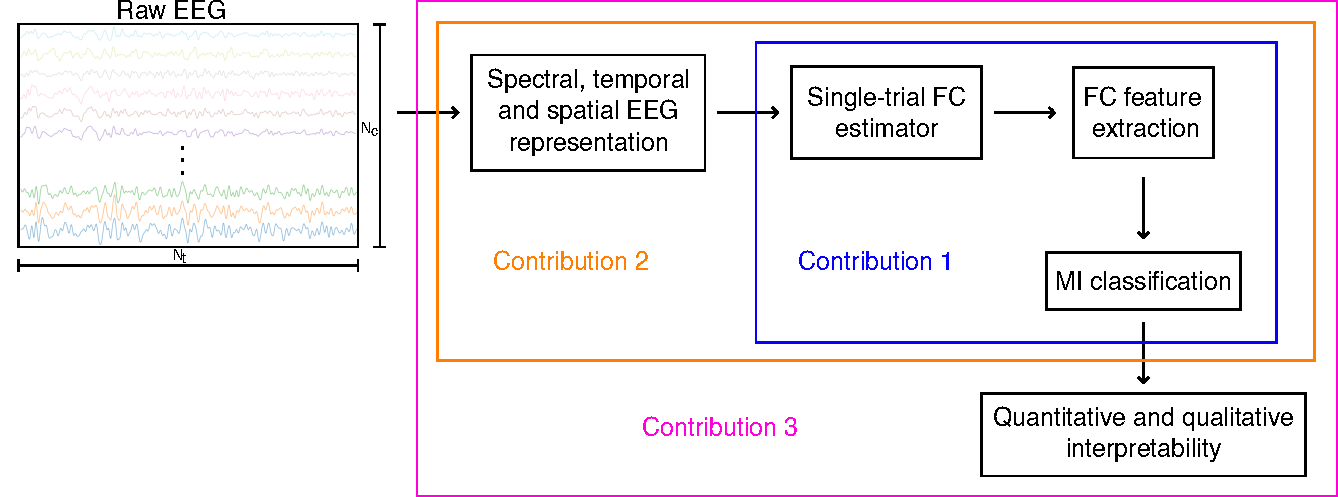
\includegraphics[scale=0.6]{Figures/outline_and_contributions/general_contributions.pdf}
    \caption{Schematic display of the main thesis contributions, including the single-trial FC estimator and feature extraction, an end-to-end approach from EEG representations to MI classification, and quantitative and qualitative strategies for model interpretation\label{fig:img_gen_outline}}
\end{figure}

This chapter offers a clear introduction to the main contributions of this thesis, as illustrated in \cref{fig:img_gen_outline}. Firstly, it presents a novel single-trial FC estimator designed to improve MI classification tasks by addressing nonlinearities, intersubject variability, and spurious connections. Secondly, it introduces a comprehensive end-to-end approach aimed at extracting subject-specific spectral, temporal, and spatial EEG representations, which can aid in reducing the incidence of artifacts and establishing more relevant connections. Lastly, the chapter suggests qualitative and quantitative interpretability strategies for comparing DL EEG-based MI-BCI models, alongside a regularization approach to further mitigate spurious connections.


\section{Single-Trial FC for Enhancing MI-BCI Classification \label{sec:contribution1}}

As referenced in \cref{sec:singlefc}, implementing robust single-trial FC estimators and streamlined feature extraction methodologies is paramount to improving the MI-BCI model's accuracy without affecting its interpretability. More specifically, successful strategies must be devised to confront the complex issues related to spurious connectivities, non-linearity, non-stationarity, and inter-subject variability. Upon a comprehensive examination of the state-of-the-art in \cref{sec:sota1}, our proposal addresses non-stationarity by implementing short sliding windows, which are presumed weakly stationary, at varying widths \cite{gaur2021sliding}. The problem of non-linearity integrating a Gaussian kernel that has proven effective against non-linear situations \cite{gunawardena2023kernel}. Specifically, we propose an extension of Bochner's theorem \cite{bochner2020harmonic}, named the Kernel-based Cross-Spectral FC (KCS-FC),  to approximate the cross-spectral distribution of a stationary kernel function by using a weighted sum of Gaussian-based pairwise relationships within different sub-band filters and time windows. The challenge of inter-subject variability using a sub-band filtering technique \cite{mammone2023autoencoder}. Moreover, a vectorization representation is proposed for FC feature extraction, mainly because of its seamless integration with end-to-end models and its responses, which are closely similar to those in CSP under linear classifier scenarios \cite{meng2023rhythmic, zoumpourlis2022covmix}. To restrict spurious connectivities, we propose introducing an elastic-net regularization mechanism \cite{tay2023elastic}. \cref{fig:contribution1} shows a graphical depiction of this proposition.  


\section{Automatic Subject-Specific EEG Representation for MI-BCI}

As referenced in \cref{sec:problem2}, it is crucial to implement models that do not strongly rely on handcrafted subject-specific EEG representations. These kinds of models can help get rid of artifacts and reduce false connections, which will make MI-BCI more accurate, especially for people who do not do well with their BCI (BCI inefficiency) \cite{park2023improving}. The following method is proposed based on the state-of-the-art exploration in \cref{sec:sota2}. First, DL strategies are proposed due to their significant efficacy in dealing with artifact removal, further mitigating the problem of spurious connectivities\cite{altaheri2023deep, huang2023discrepancy, hassanpour2019novel}. Specifically, end-to-end DL models using raw EEG as inputs are preferred as they require little or no preprocessing and allow for light architectures \cite{dose2018end, amin2019deep}. Secondly, we propose using a CNN layer to automatically extract temporal and spectral features \cite{altaheri2023deep, craik2019deep, musallam2021electroencephalography, lawhern2018eegnet}. Additionally, spatial extraction is performed by creating a custom layer incorporating the KCS-FC function from our contribution in \cref{sec:contribution1}. This contribution is illustrated in \cref{fig:contribution2}.


\section{Qualitative and Quantitative Post-Hoc and Intrinsic Explainability}

As referenced in \cref{sec:problem3}, transparency and interpretability strategies in MI-BCI models are critical in healthcare and medical decision-making scenarios \cite{miotto2018deep, xiao2018opportunities}. Additionally, measuring the effectiveness of new MI-BCI models with qualitative and quantitative explainability from multiple domains is not easy. The following explainable AI strategy is proposed based on the state-of-the-art exploration in \cref{sec:sota3}. Firstly, we propose qualitative interpretability using Layer-CAM post-hoc interpretability, which is based on the Grad-CAM method and can work with any CNN architecture \cite{chaddad2023survey}. It presents a decent accuracy location \cite{nunnari2021overlap} and highlights spatiotemporal triggers in the raw EEG. Intrinsic interpretability is achieved by checking the last layer weights, resulting in channel importance that is represented as a topoplot. Secondly, for quantitative interpretation, we borrow the concept of average drop \cite{naidu2020cam} from image processing to compare different MI-BCI models. \changes{To compare results we include a regularization technique based on Renyi's entropy to analyze how interpretability is affected when the cross-information potential of the internal FC of the KCS-FCnet is maximized}. This leads to the proposed Interpretable Regularized Kernel Cross-Spectral Functional Connectivity Network (IRKCS-FCnet) depicted in \cref{fig:contribution3}.

